\documentclass[border=3pt,tikz]{standalone}
\usepackage{amsmath}
\usetikzlibrary{calc}
\usetikzlibrary{arrows.meta} % for arrow size
\begin{document}
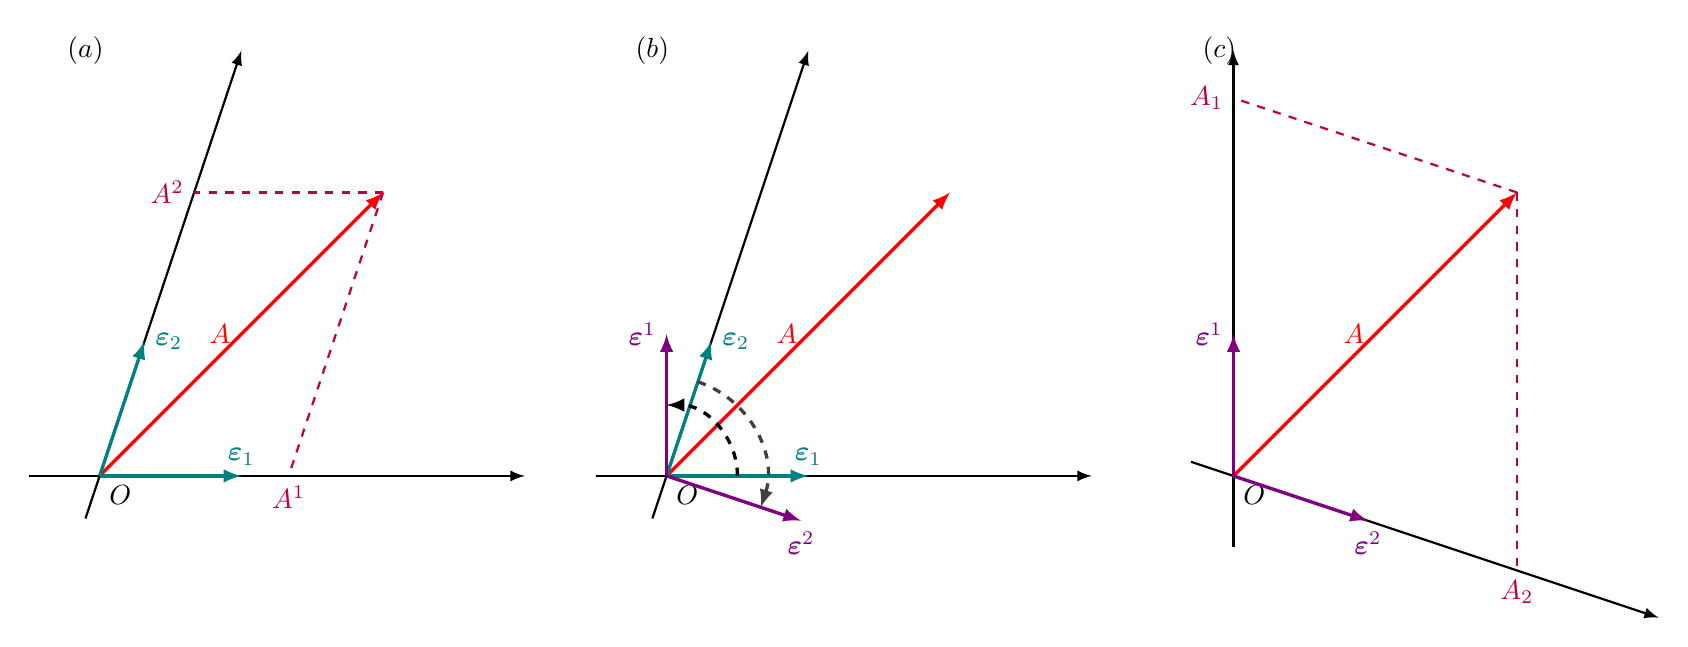
\begin{tikzpicture}[scale=1.8]
    \usetikzlibrary {arrows.meta}
    \usetikzlibrary {calc}
    \node at (-0.1, 3) {$(a)$};
    \draw[thick, -latex] (-0.5, 0) -- (3, 0);
    \draw[thick, -latex] (-0.1, -0.3) -- (1, 3);
    \draw[red, very thick, -latex] (0, 0) -- node [left] {$A$} ++ (2, 2);
    \node[below right] at (0, 0) {$O$};
    \draw[teal, very thick, -latex] (0, 0) -- (1, 0.0) node [above] {$\boldsymbol{\varepsilon}_1$};
    \draw[teal, very thick, -latex] (0, 0) -- (0.3162, 0.9487) node [right] {$\boldsymbol{\varepsilon}_2$};
    \draw[purple, thick, dashed] (2, 2) -- (0.6667, 2) node [left] {$A^2$};
    \draw[purple, thick, dashed] (2, 2) -- (1.3333, 0) node [below] {$A^1$};

    \begin{scope}[xshift=4cm]
        \node at (-0.1, 3) {$(b)$};
        \draw[thick, -latex] (-0.5, 0) -- (3, 0);
        \draw[thick, -latex] (-0.1, -0.3) -- (1, 3);
        \draw[red, very thick, -latex] (0, 0) -- node [left] {$A$} ++ (2, 2);
        \node[below right] at (0, 0) {$O$};
        \draw[teal, very thick, -latex] (0, 0) -- (1, 0.0) node [above] {$\boldsymbol{\varepsilon}_1$};
        \draw[teal, very thick, -latex] (0, 0) -- (0.3162, 0.9487) node [right] {$\boldsymbol{\varepsilon}_2$};
        \draw[violet, very thick, -latex] (0, 0) -- (0, 1) node [left] {$\boldsymbol{\varepsilon}^1$};
        \draw[violet, very thick, -latex] (0, 0) -- (0.9487, -0.3162) node [below] {$\boldsymbol{\varepsilon}^2$};
        \draw[dashed, very thick, -latex,] (0.5, 0) arc (0:90:0.5);
        \draw[dashed, darkgray, very thick, -latex,] (0.22133999999999998, 0.66409) arc (71.565:-18.435:0.7);

    \end{scope}

    \begin{scope}[xshift=8cm]
        \node at (-0.1, 3) {$(c)$};
        \draw[thick, -latex] (0, -0.5) -- (0, 3);
        \draw[thick, -latex] (-0.3, 0.1) -- (3, -1);
        \draw[red, very thick, -latex] (0, 0) -- node [left] {$A$} ++ (2, 2);
        \node[below right] at (0, 0) {$O$};
        \draw[violet, very thick, -latex] (0, 0) -- (0, 1) node [left] {$\boldsymbol{\varepsilon}^1$};
        \draw[violet, very thick, -latex] (0, 0) -- (0.9487, -0.3162) node [below] {$\boldsymbol{\varepsilon}^2$};
        \draw[purple, thick, dashed] (2, 2) -- (2, -0.666) node [below] {$A_2$};
        \draw[purple, thick, dashed] (2, 2) -- (0, 2.666) node [left] {$A_1$};
    \end{scope}
    
    \end{tikzpicture}  
\end{document}